%% LaTeX Beamer presentation template (requires beamer package)
%% see http://latex-beamer.sourceforge.net/
%% idea contributed by H. Turgut Uyar
%% template based on a template by Till Tantau
%% this template is still evolving - it might differ in future releases!

\documentclass{beamer}

\mode<presentation>
{
\usetheme{Warsaw}

\setbeamercovered{transparent}
}
\usepackage[english]{babel}
\usepackage[latin1]{inputenc}

% font definitions, try \usepackage{ae} instead of the following
% three lines if you don't like this look
\usepackage{mathptmx}
\usepackage[scaled=.90]{helvet}
\usepackage{courier} 

\usepackage{graphicx}

\usepackage[T1]{fontenc}

 
\title{Scenario Variability Management}
\subtitle{A Controlled Experiment}

\subtitle{A Controlled Experiment}

% - Use the \inst{?} command only if the authors have different
%   affiliation.
%\author{F.~Author\inst{1} \and S.~Another\inst{2}}
\author{Rodrigo Bonif\'{a}cio\inst{1} \and Paulo Borba\inst{1} \and Cristiano
Ferraz\inst{2}}

% - Use the \inst command only if there are several affiliations.
% - Keep it simple, no one is interested in your street address.
\institute[Federal University of Pernambuco]
{
\inst{1}%
Informatics Center
\and
\inst{2}%
Department of Statistics}

\date{Date / Occasion}


% This is only inserted into the PDF information catalog. Can be left
% out.
%\subject{Talks}



% If you have a file called "university-logo-filename.xxx", where xxx
% is a graphic format that can be processed by latex or pdflatex,
% resp., then you can add a logo as follows:

% \pgfdeclareimage[height=0.5cm]{university-logo}{university-logo-filename}
% \logo{\pgfuseimage{university-logo}}



% Delete this, if you do not want the table of contents to pop up at
% the beginning of each subsection:
\AtBeginSubsection[]
{
\begin{frame}<beamer>
\frametitle{Outline}
\tableofcontents[currentsection,currentsubsection]
\end{frame}
}

% If you wish to uncover everything in a step-wise fashion, uncomment
% the following command:

%\beamerdefaultoverlayspecification{<+->}

\begin{document}

\begin{frame}
\titlepage
\end{frame}

\begin{frame}
\frametitle{Outline}
\tableofcontents
% You might wish to add the option [pausesections]
\end{frame}


\section{Structured Abstract}

\begin{frame}
\frametitle{Background}
Existing approaches for scenario variability management do not present a clear
separation between \emph{variability artifacts} and \emph{use case scenarios}.
As a consequence:
\begin{itemize}
  \item (PLUC) There is no separate artficat for variability modeling; or
  \item (PLUSS) Features are directly related to use case scenarios; or 
  \item (Pauline) Scenarios are directly related to features
\end{itemize}
\end{frame}

\begin{frame}
\frametitle{Objective}

\begin{block}{Object under examination}
Compare three different techniques for scenario variability management: PLUC,
PLUSS, and SVMC. These tehcniques encompass a broad range of SoC between
variability management and scenario specifications.
\end{block}

\begin{block}{Focus}
Particularly, this comparison  is regarded to the following dimensions:
\begin{itemize}
  \item Evolvability 
  \item Traceability
  \item Product derivation?
\end{itemize}

\end{block}
  
\end{frame}

\begin{frame}
\frametitle{Method}
\framesubtitle{Layout}

We are going to use a \alert{3x3} Latin Square design. 

\begin{itemize}
  \item Groups of \alert{three students} (randomically selected)
  \item \alert{Three SPLs} used in the experiment
  \item Three techiniques (or treatments) to be compared
\end{itemize}

Each student (disposed in the rows of the squares) will be responsible for
restructuring each PL (disposed in the columns of the squares) using one
specific technique. 

\end{frame}

\begin{frame}
\frametitle{Method}
\framesubtitle{Layout}

\alert{Layout constraint:} in a given square, each treatment must be applied
only once in each row and column.

\begin{center}
\small{
\begin{tabular}{l|c|c|c}
 		& 	PL01 	& 	PL02 	& PL03 		\\ \hline
 S1   	&	SVMC    &  	PLUSS   &  PLUC		\\ \hline
 S2   	&	PLUC    &   SVMC   	&  PLUSS	\\ \hline	
 S3   	&	PLUSS   &   PLUC  	&  SVMC		\\ \hline
\end{tabular}
}
\end{center}

\alert{Replications:} In the latin square layout, the number of squares (or
groups) correspond to the number of replications --- in this experiment, this number
depends on the number of available students.

\end{frame}

\begin{frame}
\frametitle{Method}
\framesubtitle{Data collection}

\end{frame}

\begin{frame}
\frametitle{Method}
\framesubtitle{Analysis procedure}

\end{frame}

\section{Introduction}

\begin{frame}
\frametitle{Software Product Line (SPL)}

\begin{block}{Definition}
\begin{itemize}
  \item The SPL approach is a well known technique for implementing systematic
  reuse in software engineering.
  \item Based on this approach, products are customized (or generated) from a
  set of reusable assets.
\end{itemize}
\end{block}
\end{frame}

\begin{frame}
\frametitle{Software Product Line (SPL)}

\begin{block}{Technical point: variability management}
\begin{itemize}
  \item Reusable assets are extensible by means of variation points.
  \item Different techniques might be used to solve these VPs.
  \item Product decisions (capabilities) drive the generation process.
\end{itemize}
\end{block}

\center{
 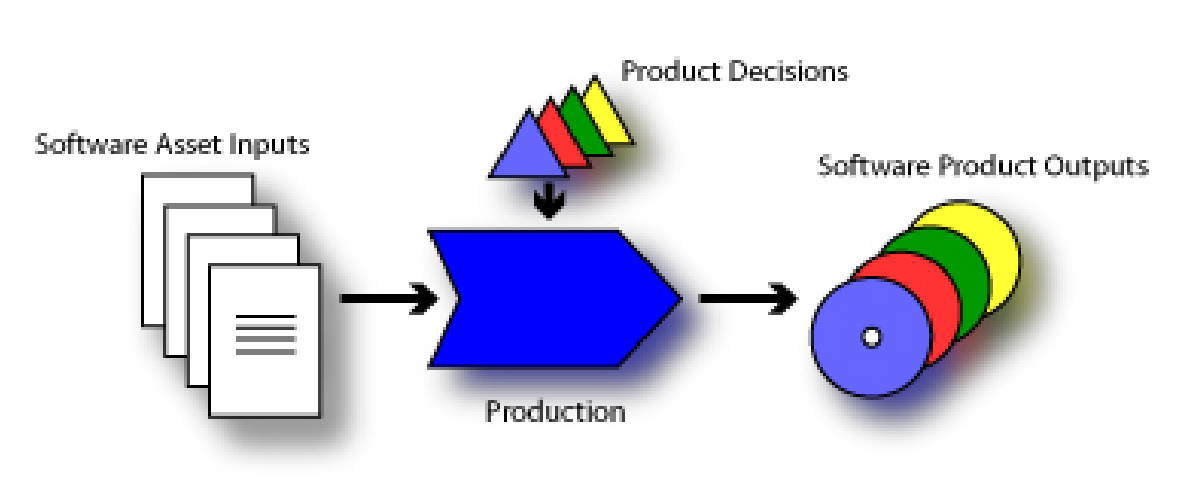
\includegraphics[scale=0.25]{img/spl.eps}
}

\end{frame}

\begin{frame}
\frametitle{Problem Statement}

\begin{block}{Field relevance}
Variability management is a complex task, since certain features (product
capabilities) require variation points to be spread in different artifacts of 
the SPLs.
\end{block}

\end{frame}

\begin{frame}
\frametitle{Problem Statement}
\begin{block}{Research problem}
\begin{itemize}
\item Different techniques for scenario variability management:
\begin{itemize} 
  \item  PLUC, PLUSS, Pauline, \ldots
\end{itemize} 

\item However, these techniques focus on the support for variation points.

\item Other issues are not weel considered:  
\begin{itemize}
  \item Evolvability 
  \item Traceability 
  \item Composability
\end{itemize}

\end{itemize}
\end{block}

\end{frame}

\begin{frame}
\frametitle{Problem statement}
\begin{block}{Proposed solution}
A new technique for representing scenario variability management. This
technique (SVMC) extends the PLUSS notation with a better separation between 
variability artifacts and scenario specifications.
\end{block}

Main contributions: 

\begin{itemize}
  \item A configuration model is used to decouple features and scenarios
  \item New mechanisms for variability management
	\begin{itemize}
      \item aspectual use cases
      \item from steps and to step clauses
    \end{itemize}   
  \item Composition processes formalized as crosscutting concerns
\end{itemize} 

\end{frame}
 
\begin{frame}
\frametitle{Experiment Objectives}

Compare different scenario variability management techniques, in order to
understand the benefits of a better separation of concerns between variability
management and scenarios specifications.

\end{frame}

\begin{frame}
\frametitle{Experiment Objectives}
\framesubtitle{Goal, Question, Metrics}

\begin{block}{Goal 1. Verify if SoC is effective to evolve SPLs} 

Question: What is the effect of SoC in the effort needed to\ldots
\small{
\begin{itemize}
  \item Q1.1. \ldots evolve the product line requirements?
  \item Q1.2. \ldots introduce a new parameter value?
  \item Q1.3. \ldots include alternative behavior?
  \item Q1.4. \ldots include optional behavior?
  \item Q1.5. \ldots change alternative behavior to optional?
  \item Q1.6. \ldots 
\end{itemize}
}
\end{block}

\end{frame}

\begin{frame}
\frametitle{Experiment Objectives}
\framesubtitle{Goal, Question, Metrics}

\begin{block}{Goal 2. Verify if SoC is effective to traceability} 

Questions:
\small{
\begin{itemize}
  \item Q2.1 How many artifacts must be reviewed in order to trace features to scenarios?
  \item Q2.2 \ldots
\end{itemize}
}
\end{block}
\end{frame}

\begin{frame}
\frametitle{Experiment Objectives}
\framesubtitle{Goal, Question, Metrics}

\begin{block}{Goal 3. Verify if SoC is effective to product generation.} 

Questions:
\small{
\begin{itemize}
  \item Does SoC contribute to reduce the effort needed to specify product
  instances?
  \item Is it possible to generate all planed products using the evaluated techniques?
  \item \ldots
\end{itemize}
}
\end{block}

\end{frame}

\begin{frame}
\frametitle{Experiment Objectives}
\framesubtitle{Goal, Question, Metrics}

\begin{block}{Additional goals}
\begin{itemize}
\item Goal 4. Relate the proposed metric suite to the previous results
\item Goal 5. Relate DSM analysis to the previous results
\end{itemize}
\end{block}

\end{frame}

 
\begin{frame}
\frametitle{Context of the Experiment}

\begin{itemize}
  \item SPLs for interactive systems (use case centric)
  \item SPLs' size: ---
  \item Subject experience: graduate and undergraduate students
  \item Treatments: PLUC, PLUSS, and SVMC
  \item Tools: ---    
\end{itemize}

\end{frame}



\section*{Summary}

\begin{frame}
\frametitle<presentation>{Summary}

\begin{itemize}
  \item The \alert{first main message} of your talk in one or two lines.
\end{itemize}

% The following outlook is optional.
\vskip0pt plus.5fill
\begin{itemize}
  \item Outlook
  \begin{itemize}
    \item Something you haven't solved.
    \item Something else you haven't solved.
  \end{itemize}
\end{itemize}
\end{frame}

\end{document}
